%% =====================================================================
%%  Information Technology & Tourism (Springer)
%%  Official article template package, December 2024 version (sn-jnl.cls v3.1)
%%  Reference style: sn-mathphys-num (numbered, natbib)
%% =====================================================================
\documentclass[pdflatex,sn-mathphys-num]{sn-jnl}

\usepackage{graphicx}
\usepackage{multirow}
\usepackage{amsmath,amssymb,amsfonts}
\usepackage{amsthm}
\usepackage{mathrsfs}
\usepackage[title]{appendix}
\usepackage{xcolor}
\usepackage{textcomp}
\usepackage{manyfoot}
\usepackage{booktabs}
\usepackage{algorithm}
\usepackage{algorithmicx}
\usepackage{algpseudocode}
\usepackage{listings}
\usepackage{url}

\raggedbottom

\begin{document}

\title[Extracting Actionable Insights from Tourism Destination Reviews]{Extracting Actionable Insights from Tourism Destination Reviews Using BERTopic and LLM-Based Aspect Sentiment Analysis at the Sentence Level}

\author*[1]{\fnm{Ahmad Fathan} \sur{Hidayatullah}}\email{fathan@uii.ac.id}

\author[2]{\fnm{Amgad} \sur{Al Ameri}}\email{23523242@students.uii.ac.id}

\author[2]{\fnm{Akram} \sur{Abdullah}}\email{23523241@students.uii.ac.id}

\author[3]{\fnm{Ardiansyah} \sur{Ardiansyah}}\email{ardiansyah@fmipa.unila.ac.id}

\affil*[1]{\orgdiv{Department of Informatics}, \orgname{Universitas Islam Indonesia}, \orgaddress{\street{}, \city{Yogyakarta}, \country{Indonesia}}}

\affil[2]{\orgdiv{Undergraduate Program in Informatics}, \orgname{Universitas Islam Indonesia}, \orgaddress{\street{}, \city{Yogyakarta}, \country{Indonesia}}}

\affil[3]{\orgdiv{Department of Computer Science}, \orgname{Universitas Lampung}, \orgaddress{\street{}, \city{Lampung}, \country{Indonesia}}}

\abstract{Online reviews are a primary source of tourism intelligence, but computational pipelines typically assign one sentiment label per review. This aggregation is convenient, yet a review that praises the scenery while criticising the road is summarised into a single polarity that matches neither statement. The size of that loss has not been quantified for Indonesian tourism reviews. This study quantifies how much aspect-level sentiment is lost when a review is treated as one unit, and develops a sentence-level framework that recovers it, combining BERTopic topic modelling with large language model (LLM) aspect-based sentiment analysis (ABSA) applied to individual sentences. A computational study was conducted on 1,530 Google Maps reviews from 34 tourist destinations in Yogyakarta, Indonesia. Reviews were split into 6,552 sentences with a round-trip-validated, slice-based splitter. Aspect extraction used Qwen2.5-7B-Instruct in 4-bit NF4 quantisation under greedy decoding, with a closed 12-aspect taxonomy and an evidence-span requirement: every extracted keyword must appear verbatim in the sentence it is attributed to. Of 6,479 labelled sentences, 5,170 (79.8\%) carried at least one aspect and 8,412 aspect mentions were extracted, or 5.50 per review against 3.72 for the same corpus analysed at review level. Aggregation hides structure: 2,144 sentences (33.1\%) discuss two or more aspects and 411 of those (19.2\%) are internally contradictory, and 42.3\% of reviews with mentions carry both positive and negative aspects. Re-extraction at sentence level reverses the sign of three aspects: safety ($-0.24$), accessibility ($-0.10$) and crowd level ($-0.02$) are net negative, whereas review-level aggregation scored all three positive. The contribution is evidence about the unit of analysis rather than a new sentiment model: aggregation, not model capability, governs what is visible in review analytics. No human-annotated gold standard was constructed, so no accuracy claim is made.}

\keywords{Tourism reviews, Aspect-based sentiment analysis, Large language models, BERTopic, Sentence-level analysis, Indonesia}

\maketitle

\section{Introduction}\label{sec1}

Tourism is one of the main drivers of economic growth worldwide. It can contribute to regional income, employment creation, and cultural preservation. As the industry becomes increasingly competitive, tourist destinations must continually adapt to evolving visitor expectations to remain attractive to both domestic and international visitors. The sustainability and competitiveness of tourism destinations increasingly depend on stakeholders' ability to understand visitor experiences and expectations in a data-driven manner.

In recent years, the growth of social media platforms and location-based services such as Google Maps has transformed the way tourists share feedback and evaluate destinations. Online reviews have become a primary source of information for travellers when planning trips, offering spontaneous, experience-based opinions that reflect real visitor perceptions \cite{bib1}.

However, the massive volume of online reviews poses a significant challenge, as popular tourist attractions can accumulate thousands of reviews, leading to information overload for both tourists and destination managers \cite{bib2}. In addition to being numerous, reviews are often unstructured and multilingual \cite{bib3,bib4}. They can be anything from long, detailed accounts of experiences to short, vague comments. It is not possible to manually extract useful and actionable insights from such diverse data, so automated analysis methods are necessary for good tourism management.

To address these challenges, topic modelling and aspect-based sentiment analysis (ABSA) offer complementary solutions. Topic modelling automatically uncovers latent thematic patterns from large collections of unstructured reviews, while ABSA goes further by identifying specific aspects and determining sentiment toward each independently, unlike general sentiment analysis, which produces only a single polarity score. Together, they enable stakeholders to pinpoint both dominant topics and specific areas for improvement. A further assumption is usually left implicit: that the review is the natural unit of analysis. This assumption is questionable for narrative reviews, in which a single text often praises one dimension while criticising another. When such a review is aggregated into one label, the resulting polarity describes neither statement.

The main objectives of this study are as follows: (1) to identify latent thematic patterns using BERTopic, (2) to implement LLM-based ABSA for Indonesian tourism reviews, (3) to quantify how much aspect-level information a review-level formulation discards, and (4) to derive actionable insights from the recovered sentence-level structure. The contribution is therefore not a new sentiment model but evidence about the unit of analysis: the same corpus, read at sentence level, reverses the sign of three of its twelve aspects.

\section{Literature Review}\label{sec2}

The intersection of topic modelling and sentiment analysis for tourism review mining has attracted growing scholarly attention. Several studies have employed traditional topic modelling combined with lexicon-based sentiment analysis. Singh et al.\ \cite{bib6} analysed over 104,000 TripAdvisor reviews from Indian tourist destinations using AFINN lexicon-based sentiment analysis and Non-Negative Matrix Factorization (NMF) for topic modelling, revealing ``Joy'' as the predominant emotion. Similarly, Ali et al.\ \cite{bib7} combined LDA with VADER and TextBlob for aspect-level sentiment identification on Marrakech attractions, achieving 77.3\% accuracy. Balasubramanian et al.\ \cite{bib8} employed the Syuzhet package in R with LDA to analyse post-COVID-19 tourist concerns, identifying dominant emotions across travel stages. However, these lexicon-based approaches share common limitations including inability to detect sarcasm and contextual nuances.

Machine learning approaches have demonstrated improved classification performance. Masrury et al.\ \cite{bib9} achieved 88--91\% accuracy using a Na\"ive Bayes classifier with LDA for mobile application quality assessment. Mishra et al.\ \cite{bib10} employed LSTM-RNN deep learning with VADER and LDA on COVID-19 tourism tweets, achieving 80.9\% test accuracy for hospitality sentiment classification. A study by Carvache-Franco et al.\ \cite{bib11} examined COVID-19 tourism discourse using chi-square-based word association and SentiStrength, demonstrating Twitter's role in crisis communication despite temporal limitations.

With the emergence of transformer-based approaches, some studies applied topic modelling and transformer-based models to analyse tourism reviews. The introduction of transformer architectures, most notably BERT, and the development of efficient sentence-level representations through Sentence-BERT \cite{bib12} enabled a new generation of semantically rich models suited to ABSA tasks. Reimers and Gurevych \cite{bib13} further extended this work by producing multilingual sentence embeddings via knowledge distillation, enabling high-quality semantic representations across languages, a critical capability for analysing Indonesian user-generated content. Building on this foundation, Li et al.\ \cite{bib14} demonstrated that ABSA of customer-generated online reviews can yield fine-grained predictive insights relevant to tourism management, applying the technique to restaurant survival prediction. Vi\~n\'an-Lude\~na and De Campos \cite{bib15} evaluated tourist dissatisfaction across social media platforms using ABSA, finding that a granular aspect-level view consistently outperforms document-level sentiment in actionability for destination managers.

Rutba and Pramana \cite{bib16} utilised pre-trained BERT models for aspect-based sentiment analysis combined with LDA, revealing sentiment patterns associated with specific tourism destinations. D\'iaz-Pacheco et al.\ \cite{bib17} proposed a comprehensive deep-learning-based method (CDLM-ITT) that integrates embedding-based clustering via Sentence Transformers and UMAP for topic modelling, GPT-3 for automated topic labelling, and lexicon-based polarity classification to analyse tourism-related textual data at scale.

More recent studies have explored transformer-based models with zero-shot and prompted learning capabilities. Nawawi et al.\ \cite{bib5} integrated aspect-based sentiment analysis with zero-shot learning using pretrained RoBERTa for keyword extraction and K-means clustering for aspect construction, effectively analysing tourist experiences without extensive annotated datasets. The emergence of large language models has expanded the possibilities for such analysis. Krugmann and Hartmann \cite{bib18} benchmarked GPT-3.5, GPT-4 and Llama 2 against established transfer learning models on sentiment tasks, reporting that LLMs in a zero-shot setting can approach fine-tuned classifiers when labelled training data are scarce. Zhang et al.\ \cite{bib19} conducted a comprehensive assessment of LLMs across sentiment analysis sub-tasks, including ABSA, and found that coarser polarity tasks are handled well while structured aspect-level extraction remains more demanding. These results motivate a constrained prompt design in the present study: a closed aspect list, an explicit output schema, and a requirement that every keyword be copied from the source sentence.

The pairing of neural topic modelling with LLM-based sentiment analysis has begun to appear in the literature. Jeong and Lee \cite{bib21} pioneered a methodology closely related to the present study by combining ChatGPT-based ABSA with BERTopic to explore hotel service failures on TripAdvisor, demonstrating that the combination of LLM-generated aspect summaries and BERTopic topic modelling yields richer, more interpretable insights than either approach alone. Their work confirms the complementary value of these two analytical layers: topic modelling reveals latent thematic structures while LLM-based ABSA provides granular sentiment attribution within each theme.

Despite these contributions, several gaps remain. Most studies rely on supervised or lexicon-based methods requiring domain-specific training data, limiting adaptability to new contexts. Traditional topic modelling approaches like LDA also struggle to capture semantic relationships effectively. Few studies have combined LLM-based ABSA with neural topic modelling techniques like BERTopic that leverage transformer embeddings for improved topic coherence \cite{bib22}. Furthermore, research focusing on Indonesian-language tourism reviews remains limited, despite the multilingual and code-switching challenges unique to user-generated content in this context. This study addresses these gaps by integrating prompted ABSA using Qwen2.5-7B-Instruct with BERTopic-based topic modelling, underpinned by multilingual sentence embeddings, providing a flexible and resource-efficient framework for analysing tourism reviews.

\section{Research Methodology}\label{sec3}

This study employs a computational approach combining BERTopic modelling with LLM-based ABSA. As shown in Fig.~\ref{fig1}, the framework consists of four stages: (1) review collection from Google Maps across 34 destinations in the Yogyakarta region; (2) sentence-level splitting of each review so that aspects are attributed to the sentence that carries them rather than to the review as a whole; (3) aspect and sentiment extraction with a locally executed Qwen2.5-7B-Instruct model constrained to a 12-aspect glossary; and (4) aggregation of mentions by aspect, destination and polarity. Stage 2 is the methodological difference from prior work, which extracts aspects once per review.

\begin{figure}[htbp]
\centering
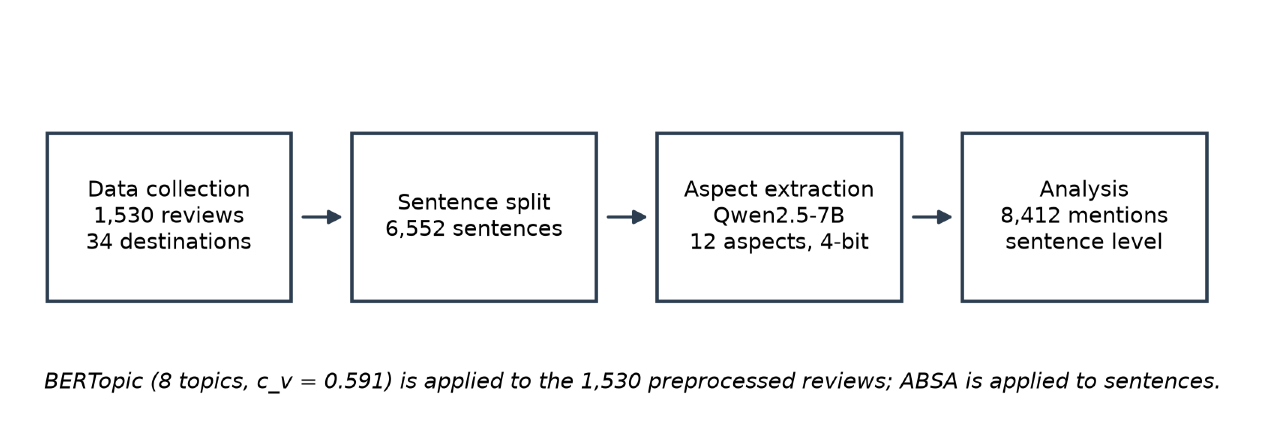
\includegraphics[width=\textwidth]{figures/fig1_workflow.pdf}
\caption{Research workflow: reviews, sentence splitting, aspect extraction and sentence-level analysis.}\label{fig1}
\end{figure}

\subsection{Data Collection}\label{subsec1}

Data were collected from Google Reviews for tourist destinations in Yogyakarta, a major cultural and educational tourism hub in Indonesia. The destination list was compiled from yogyes.com, a local tourism portal, yielding 34 destinations across eight categories: beaches, temples, cultural sites, museums, nature, historical sites, religious sites and agrotourism, as summarised in Table~\ref{tab1}. Beaches dominate the corpus, accounting for 18 of the 34 destinations.

\begin{table}[htbp]
\caption{Tourist destination categories in Yogyakarta with examples}\label{tab1}
\begin{tabular}{@{}ll@{}}
\toprule
Category & Tourist Destination Example\\
\midrule
Beaches & Pantai Parangtritis, Pantai Indrayanti, Pantai Baron, Pantai Drini, Pantai Kukup\\
Temples & Candi Prambanan, Candi Kalasan, Candi Mendut\\
Cultural Sites & Tugu Jogja, Alun-alun Kidul, Prawirotaman, Malioboro\\
Museums & Museum Ullen Sentalu, Monumen Jogja Kembali, Studio Alam Gamplong\\
Nature & Gumuk Pasir Parangkusumo, Bukit Bintang, Pantai Wediombo\\
Historical & Makam Raja-Raja Imogiri, Situs Warungboto\\
Religious & Sendang Sono\\
Agrotourism & Agrowisata Bhumi Merapi\\
\botrule
\end{tabular}
\end{table}

Reviews were extracted using Playwright, a browser-based automation tool, collecting up to 100 reviews per destination and producing an initial dataset of approximately 3,000 reviews. These reviews, primarily written in Bahasa Indonesia, frequently incorporate informal expressions, local slang and English terms, reflecting the multilingual and code-switching tendencies typical of Indonesian user-generated content. Table~\ref{tab2} presents sample reviews with their star ratings.

\begin{table}[htbp]
\caption{Sample tourist destination reviews with star ratings}\label{tab2}
\begin{tabular}{@{}p{2.2cm}p{9.6cm}c@{}}
\toprule
Destination & Review Text & Stars\\
\midrule
Candi Prambanan & Wonderful experience. Tempat bersejarah yang penuh dengan nilai historis dan berdiri dengan arsitektur yang sangat indah. Such an amazing place. & 5\\
Museum Ullen Sentalu & Bagus si. Cocok buat orang yg suka sama sejarah. Ada 3 jenis tiket, paling murah 50rb, 60rb sama 100rb. Lokasinya jauh banget di dataran tinggi. & 4\\
Prawirotaman & Jalanannya bagus banyak cafe dan nuansanya mirip legian bali di malam hari. Yg gila parkirnya 10rb mahal banget! & 3\\
Malioboro & Ramenya oke. Makanan susah nemu yg enak. 80\% SELALU HIRUP ASAP ROKOK. Tolong diperketat lagi! & 2\\
Pantai Drini & Sebenernya pantainya indah, sayang para pedagang payung dan tikar yg merusak suasana. & 1\\
\botrule
\end{tabular}
\end{table}

\subsection{Data Preprocessing}\label{subsec2}

Text preprocessing proceeded in four stages. First, exact-text duplicate removal reduced the dataset by 49\%, from 3,000 to 1,530 unique reviews. Second, text cleaning applied lowercase conversion and removed URLs, email addresses and digits. Third, punctuation and special characters were removed. Fourth, stop-word removal applied a combined list of 453 words: 255 unique Indonesian stop words defined in the preprocessing module and the 198 English stop words supplied by NLTK. Table~\ref{tab3} presents the dataset statistics after preprocessing.

\begin{table}[htbp]
\caption{Dataset statistics}\label{tab3}
\begin{tabular}{@{}lr@{}}
\toprule
Metric & Value\\
\midrule
Total destinations & 34\\
Original reviews collected & $\sim$3,000\\
After deduplication & 1,530\\
Deduplication rate & 49\%\\
Average star rating & 4.68/5\\
5-star reviews & 78.6\%\\
\botrule
\end{tabular}
\end{table}

\subsection{Topic Modelling with BERTopic}\label{subsec3}

BERTopic is a neural topic modelling framework that leverages pre-trained transformer-based embeddings to generate coherent and semantically meaningful topic representations \cite{bib22}. Unlike traditional topic models such as Latent Dirichlet Allocation (LDA), which rely on bag-of-words representations, BERTopic operates through a modular pipeline that begins by generating dense document embeddings using Sentence-BERT (SBERT), capturing rich semantic relationships between texts. These high-dimensional embeddings are then projected into a lower-dimensional space using Uniform Manifold Approximation and Projection (UMAP), preserving both local and global structure while making the data amenable to clustering. HDBSCAN is subsequently applied to identify dense clusters of semantically similar documents, with the advantage of automatically determining the number of clusters and allowing outlier documents to remain unassigned. A class-based TF-IDF (c-TF-IDF) weighting scheme then extracts the most representative terms for each topic by measuring word importance relative to the cluster rather than individual documents. This modular architecture allows each component to be independently configured or replaced, and enables BERTopic to produce interpretable topics particularly for short and noisy texts such as online reviews. Fig.~\ref{fig2} shows the topic modelling steps in BERTopic.

\begin{figure}[htbp]
\centering
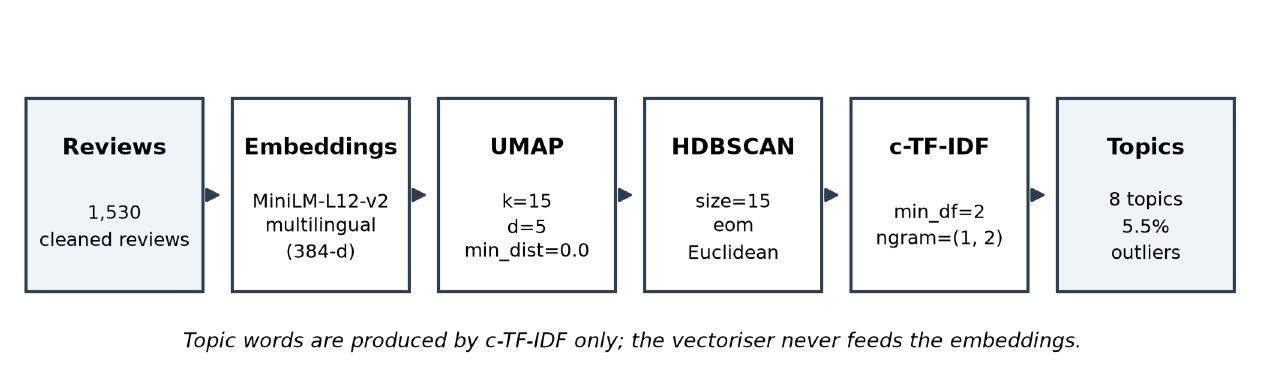
\includegraphics[width=\textwidth]{figures/fig2_bertopic.pdf}
\caption{BERTopic pipeline. Parameters are those of the final model (\texttt{min\_cluster\_size=15}, \texttt{eom}).}\label{fig2}
\end{figure}

In this study, BERTopic was configured with the following components:
\begin{itemize}
\item Document embeddings using \texttt{paraphrase-multilingual-MiniLM-L12-v2}, a multilingual Sentence-BERT model suitable for Indonesian text;
\item Dimensionality reduction using UMAP with \texttt{n\_neighbors=15}, \texttt{n\_components=5}, \texttt{min\_dist=0.0} and cosine metric;
\item Clustering using HDBSCAN with \texttt{min\_cluster\_size=15}, Euclidean metric and the excess of mass (\texttt{eom}) cluster selection method;
\item Topic representation using CountVectorizer with \texttt{min\_df=2} and \texttt{ngram\_range=(1,2)} to capture both unigrams and bigrams, with additional Indonesian stop words applied.
\end{itemize}

The configuration was selected from ten candidate settings by maximising topic coherence rather than left at its default. Probability calculation was enabled to allow soft topic assignments for downstream analysis.

\subsection{LLM-Based Aspect Sentiment Analysis}\label{subsec4}

In this study, we defined 12 tourism-specific aspects based on dimensions commonly discussed in tourism review literature and recurring in Indonesian travel reviews: cleanliness, facilities, price/value, service, accessibility, scenery/view, atmosphere, food and beverage, safety, crowd level, photo spots, and historical/cultural value. The taxonomy is closed: an aspect absent from this list cannot be reported, a restriction revisited in Section~\ref{sec6}.

Unlike prior work that assigns one label per review, ABSA here operates on sentences. Each review was split into sentences by a slice-based splitter that returns character spans of the original text rather than re-joined tokens, so every sentence is a literal substring of its review. Splitter rules: a period is not a boundary when preceded by ``Rp'', a bullet character forces a hard boundary, and no boundary may fall inside a numeric token such as ``5.000''. The splitter was validated on all 1,530 reviews: 0 round-trip failures, 164 of 164 thousand-separated prices preserved intact, and 0 sentences failing the substring test, producing 6,552 sentences. Sentences containing no letter character (for example emoji-only or numeric-only strings) were excluded from labelling, leaving 6,479.

\begin{figure}[htbp]
\centering
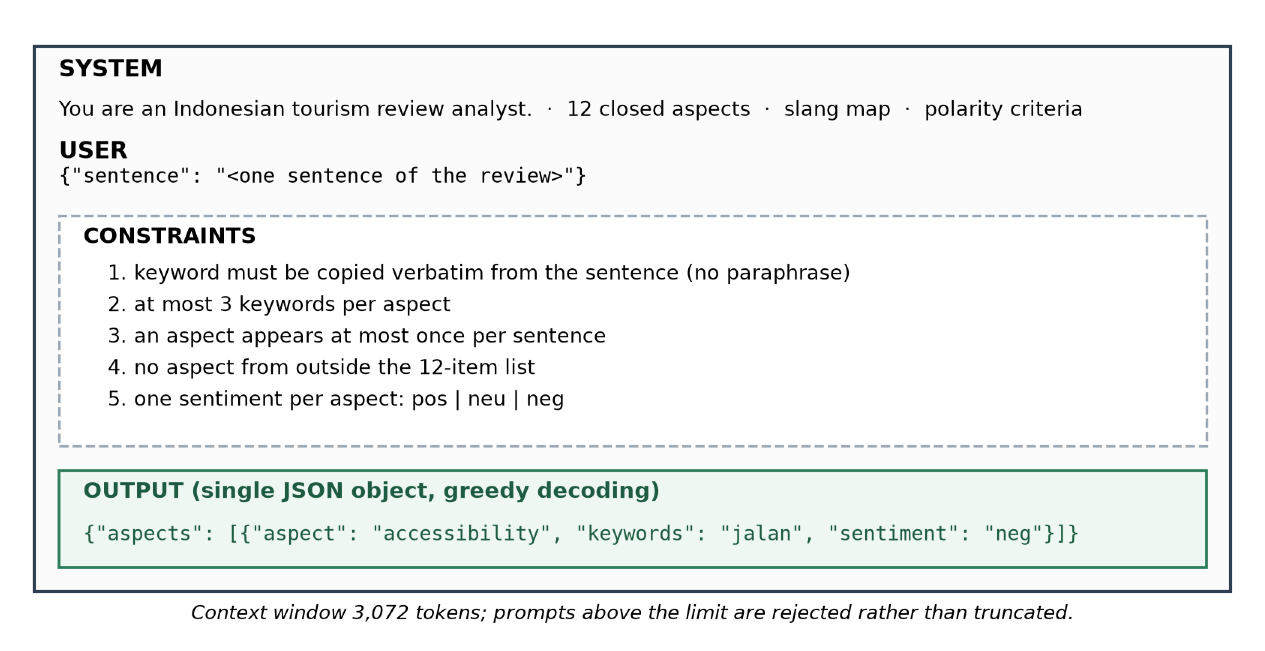
\includegraphics[width=\textwidth]{figures/fig3_prompt.pdf}
\caption{Prompt structure for aspect extraction. Every keyword must be copied verbatim from the sentence.}\label{fig3}
\end{figure}

Aspect extraction used Qwen2.5-7B-Instruct in 4-bit NF4 quantisation with double quantisation, running on a single consumer GPU. Decoding was greedy (\texttt{do\_sample=False}, \texttt{num\_beams=1}), so the pipeline is deterministic and a repeated run reproduces the same output. The prompt has three components: (1) a system instruction defining the role as an Indonesian tourism sentiment analyser, with explicit polarity criteria; (2) Indonesian slang mappings for informal expressions; and (3) the closed 12-aspect list with an output schema specifying aspect, keyword span and sentiment. Three requirements constrain the output: the keyword span must be copied verbatim from the input sentence, at most three keywords may be returned per aspect, and an aspect may be named only once per sentence. The context window was set to 3,072 tokens after truncation was found to corrupt prompts; prompts exceeding the limit are rejected rather than truncated. Fig.~\ref{fig3} shows the prompt structure.

The sentiment score for an aspect is computed as
\begin{equation}
S_a = \frac{P_a - N_a}{T_a},\label{eq1}
\end{equation}
where $S_a$ is the sentiment score for aspect $a$, $P_a$ the number of positive mentions, $N_a$ the number of negative mentions and $T_a$ the total number of mentions for that aspect. The score ranges from $-1.0$ to $+1.0$. Scores were categorised into five levels as shown in Table~\ref{tab4}.

\begin{table}[htbp]
\caption{Sentiment score interpretation ranges}\label{tab4}
\begin{tabular}{@{}ll@{}}
\toprule
Score Range & Interpretation\\
\midrule
$+0.7$ to $+1.0$ & Excellent (strong positive sentiment)\\
$+0.3$ to $<+0.7$ & Good (moderate positive sentiment)\\
$0.0$ to $<+0.3$ & Mixed (slight positive or balanced)\\
$-0.3$ to $<0.0$ & Concerning (slight negative sentiment)\\
$-1.0$ to $<-0.3$ & Poor (strong negative sentiment)\\
\botrule
\end{tabular}
\end{table}

\section{Results}\label{sec4}

\subsection{Topic Modelling Results}\label{subsec5}

The 1,530 preprocessed reviews yielded 8 topics. A total of 1,446 reviews (94.5\%) were assigned to a topic and 84 (5.5\%) remained unassigned as outliers. Coherence was $c_v = 0.5912$ and $c_{npmi} = 0.087$, computed over the eight topics. The largest topic (T0, 797 reviews, 52.1\%) is a beach and coastal cluster; T1 (450 reviews, 29.4\%) groups urban and photo-oriented visits. The remaining six topics are small and highly specific: museums and guided tours (T2), Yogyakarta city landmarks (T3), temple complexes (T4), pilgrimage sites (T5), royal burial sites (T6) and sand-dune jeep tours (T7). Because topics are derived from the same 1,530 reviews and topic assignment is not disjoint per sentence, topic identity is used descriptively and is not cross-tabulated against aspect sentiment in this study.

Fig.~\ref{fig4} shows the topic composition and Fig.~\ref{fig5} the most representative terms per topic. The eight topics resolve into four interpretable groupings rather than the five thematic pillars commonly assumed for Yogyakarta: a dominant coastal cluster (T0, T7), an urban and photography cluster (T1, T3), a heritage cluster (T2, T4, T6) and a pilgrimage cluster (T5). Culinary tourism does not emerge as an independent topic under these settings. It appears instead inside the coastal cluster, where seafood and \textit{warung} vocabulary co-occurs with beach vocabulary. The absence of a standalone culinary topic is a property of this corpus and configuration, not evidence that food is unimportant: at sentence level, food and beverage receives 662 aspect mentions, ranking sixth of twelve. Fig.~\ref{fig6} reports how that topic share is distributed across the sixteen most-reviewed destinations.

\begin{figure}[htbp]
\centering
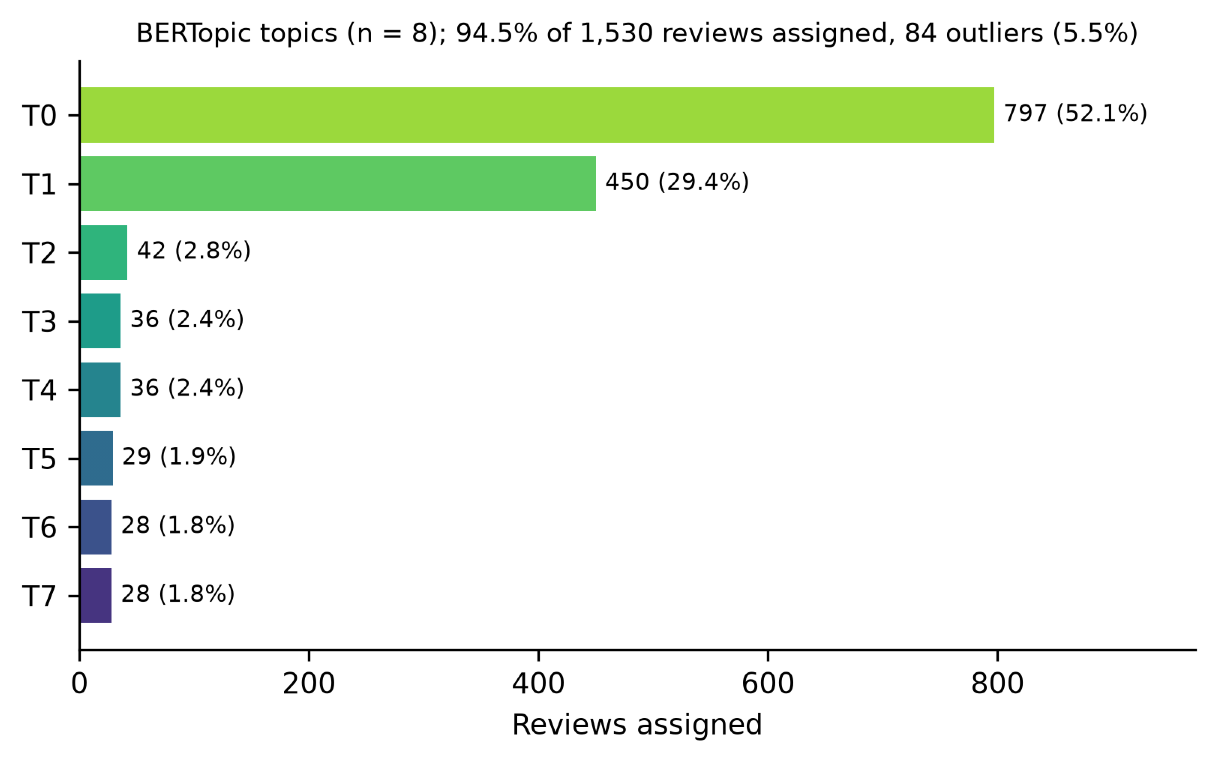
\includegraphics[width=0.95\textwidth]{figures/fig4_topic_sizes.pdf}
\caption{Topic composition: 8 topics, 94.5\% of reviews assigned, 84 outliers (5.5\%).}\label{fig4}
\end{figure}

\begin{figure}[htbp]
\centering
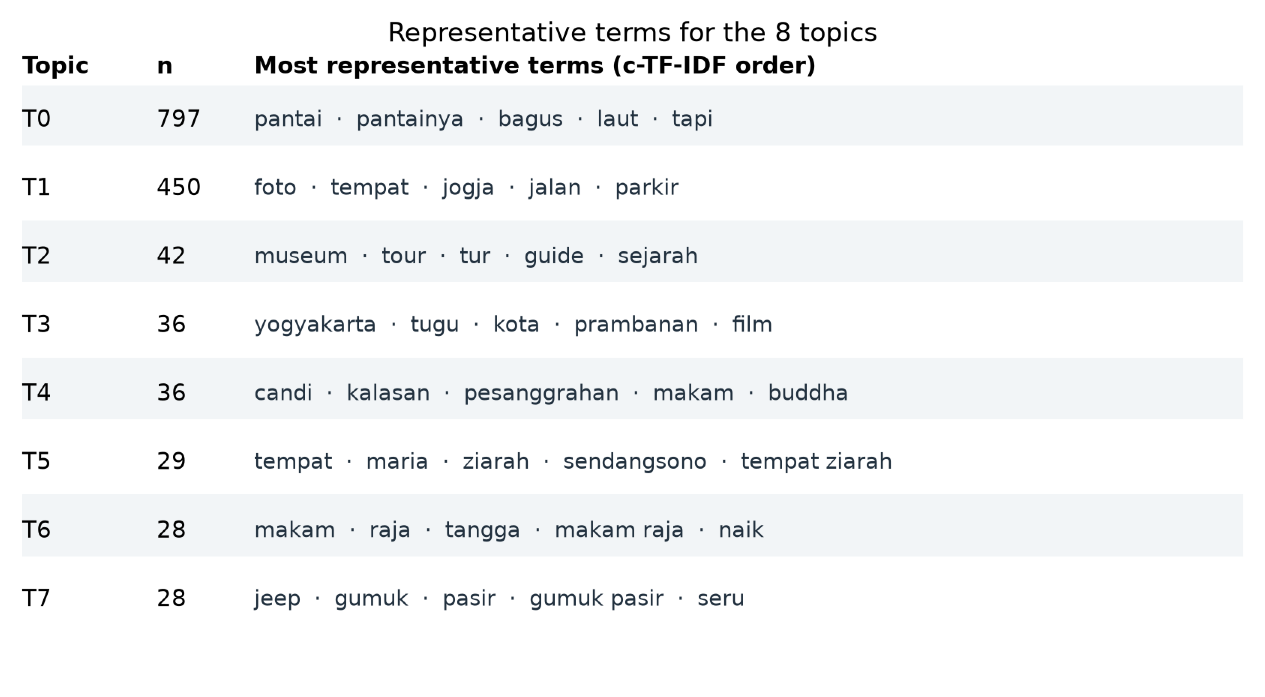
\includegraphics[width=\textwidth]{figures/fig5_topic_words.pdf}
\caption{Most representative terms for each of the eight topics.}\label{fig5}
\end{figure}

\begin{figure}[htbp]
\centering
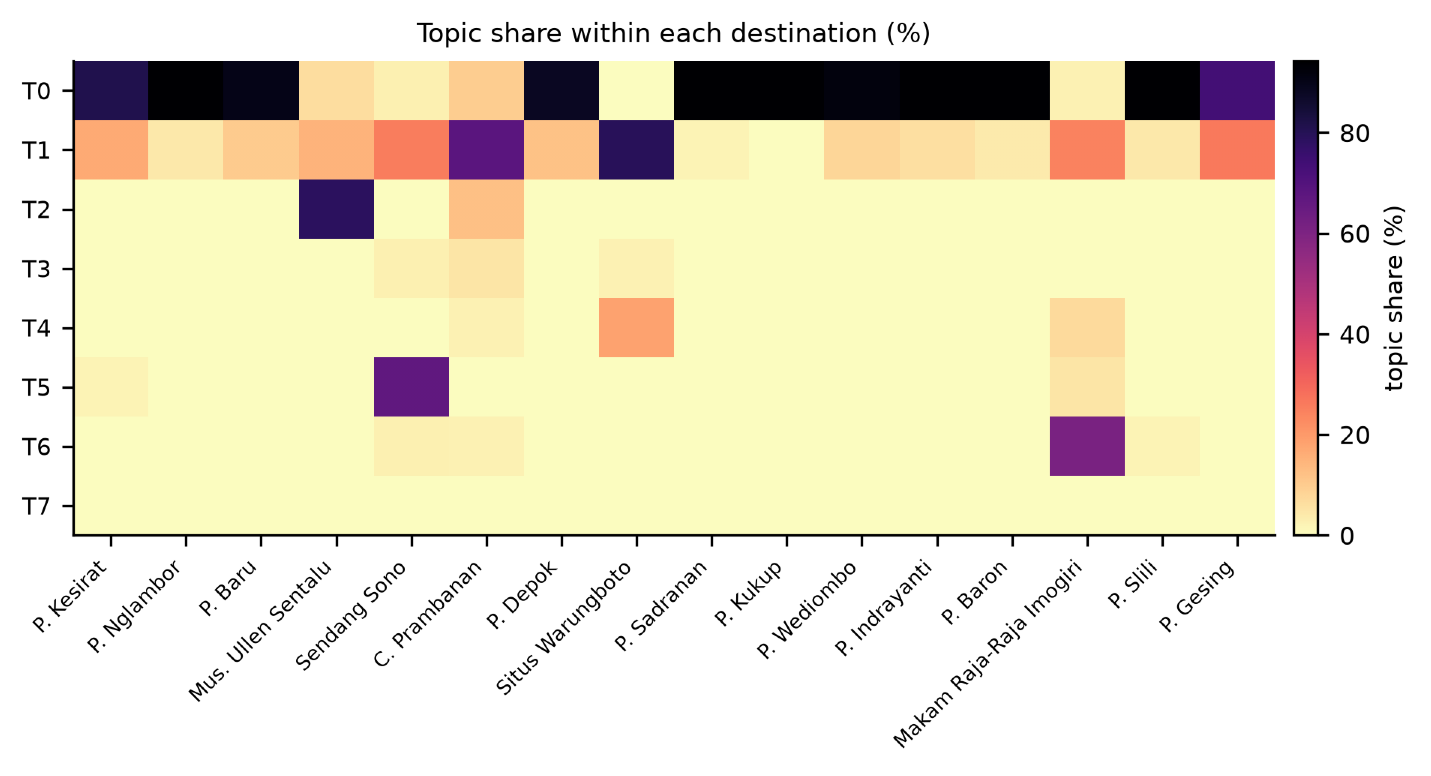
\includegraphics[width=\textwidth]{figures/fig6_topic_destination.pdf}
\caption{Share of each topic within the 16 most-reviewed destinations.}\label{fig6}
\end{figure}

\subsection{LLM-Based Sentiment Analysis Results}\label{subsec6}

At sentence level the pipeline extracted 8,412 aspect mentions from 6,479 labelled sentences, an average of 1.30 mentions per sentence and 5.50 per review. The review-level formulation applied to the same corpus produced 3.72 mentions per review, so sentence-level extraction recovers 1.48 times as many distinct judgements. Of the 6,479 sentences, 5,170 (79.8\%) contained at least one aspect. The remaining 1,309 (20.2\%) were retained in the dataset with an explicit reason code but without aspect labels: 1,205 received an empty aspect list from the model, and 104 contained an aspect outside the 12-item taxonomy whose polarity was preserved separately (Section~\ref{subsec7}). Across the 8,412 mentions, 45.8\% were positive, 37.8\% neutral and 16.4\% negative. The neutral share is high because a mention is neutral when the sentence names an aspect without evaluating it, for example when describing opening hours.

Table~\ref{tab5} reports the distribution for all 12 aspects, ordered by mention volume. Scenery/view is discussed most often (1,277 mentions), followed by atmosphere (1,112), price/value (941), facilities (900) and accessibility (883). Safety (313), service (335) and cleanliness (375) are discussed least. Scenery/view and atmosphere are also the most polarised in the positive direction: 65.2\% and 73.3\% of their mentions are positive respectively, and net scores reach $+0.59$ and $+0.63$. Photo spots ($+0.45$), cleanliness ($+0.37$), service ($+0.37$) and historical value ($+0.35$) follow.

Three aspects are net negative at sentence level: safety ($-0.24$), accessibility ($-0.10$) and crowd level ($-0.02$). Safety is the clearest case: 51.8\% of its 313 mentions are negative, concentrated in beach destinations and expressed through wave and current vocabulary. Accessibility carries the largest absolute negative volume of any aspect (313 negative mentions of 883), driven by road conditions, distance and parking. Crowd level is nearly balanced (121 positive, 129 negative, 191 neutral), and its net score close to zero should be read as an average over opposed experiences rather than as indifference. These three aspects score positive under review-level aggregation; the sign reversal is analysed in Section~\ref{subsec9}.

Sentence-level extraction makes visible a structure that review-level labelling cannot represent. Of the 6,479 labelled sentences, 2,144 (33.1\%) carry two or more aspect mentions. Within that group, 411 sentences (19.2\%) contain at least one positive and one negative aspect, so a single label applied to the sentence would be wrong about part of it. These 411 are not concentrated in negative reviews: 382 (92.9\%) occur in four- and five-star reviews, where a favourable overall verdict coexists with a specific complaint.

At review level, 1,488 reviews contain at least one aspect mention; of these, 630 (42.3\%) contain both positive and negative aspects. Any review-level representation must compress those 630 into one value, discarding the identity of whichever aspect loses. The sentence-level representation keeps both, and Table~\ref{tab5} is the direct consequence: the same corpus that appears overwhelmingly positive in aggregate contains three aspects with negative net scores.

Fig.~\ref{fig4}--\ref{fig6} present the topic layer and Fig.~\ref{fig7} the aspect layer. The two layers disagree informatively. First, volume and polarity are independent: price/value receives 941 mentions but 61.0\% of them are neutral, so a frequently discussed aspect need not be a polarised one. Second, the three negative aspects are negative by a clear margin in their own mention pools (safety $-0.24$, accessibility $-0.10$, crowd level $-0.02$), not because a few reviews dominate.

\begin{table}[htbp]
\caption{Aspect-level sentiment analysis results at sentence level}\label{tab5}
\begin{tabular*}{\textwidth}{@{\extracolsep\fill}lrrrrr}
\toprule
Aspect & Mentions & Positive (\%) & Negative (\%) & Neutral (\%) & Score\\
\midrule
Scenery/View & 1,277 & 65.2 & 6.3 & 28.5 & $+0.590$\\
Atmosphere & 1,112 & 73.3 & 10.3 & 16.5 & $+0.630$\\
Price/Value & 941 & 27.6 & 11.4 & 61.0 & $+0.163$\\
Facilities & 900 & 31.7 & 16.1 & 52.2 & $+0.156$\\
Accessibility & 883 & 25.9 & 35.4 & 38.6 & $-0.095$\\
Food \& Beverage & 662 & 34.9 & 8.9 & 56.2 & $+0.260$\\
Photo Spots & 600 & 54.5 & 10.0 & 35.5 & $+0.445$\\
Historical Value & 573 & 40.3 & 5.4 & 54.3 & $+0.349$\\
Crowd Level & 441 & 27.4 & 29.3 & 43.3 & $-0.018$\\
Cleanliness & 375 & 65.3 & 28.8 & 5.9 & $+0.365$\\
Service & 335 & 57.3 & 20.3 & 22.4 & $+0.370$\\
Safety & 313 & 27.8 & 51.8 & 20.4 & $-0.240$\\
\midrule
Overall & 8,412 & 45.8 & 16.4 & 37.8 & ---\\
\botrule
\end{tabular*}
\end{table}

\begin{figure}[htbp]
\centering
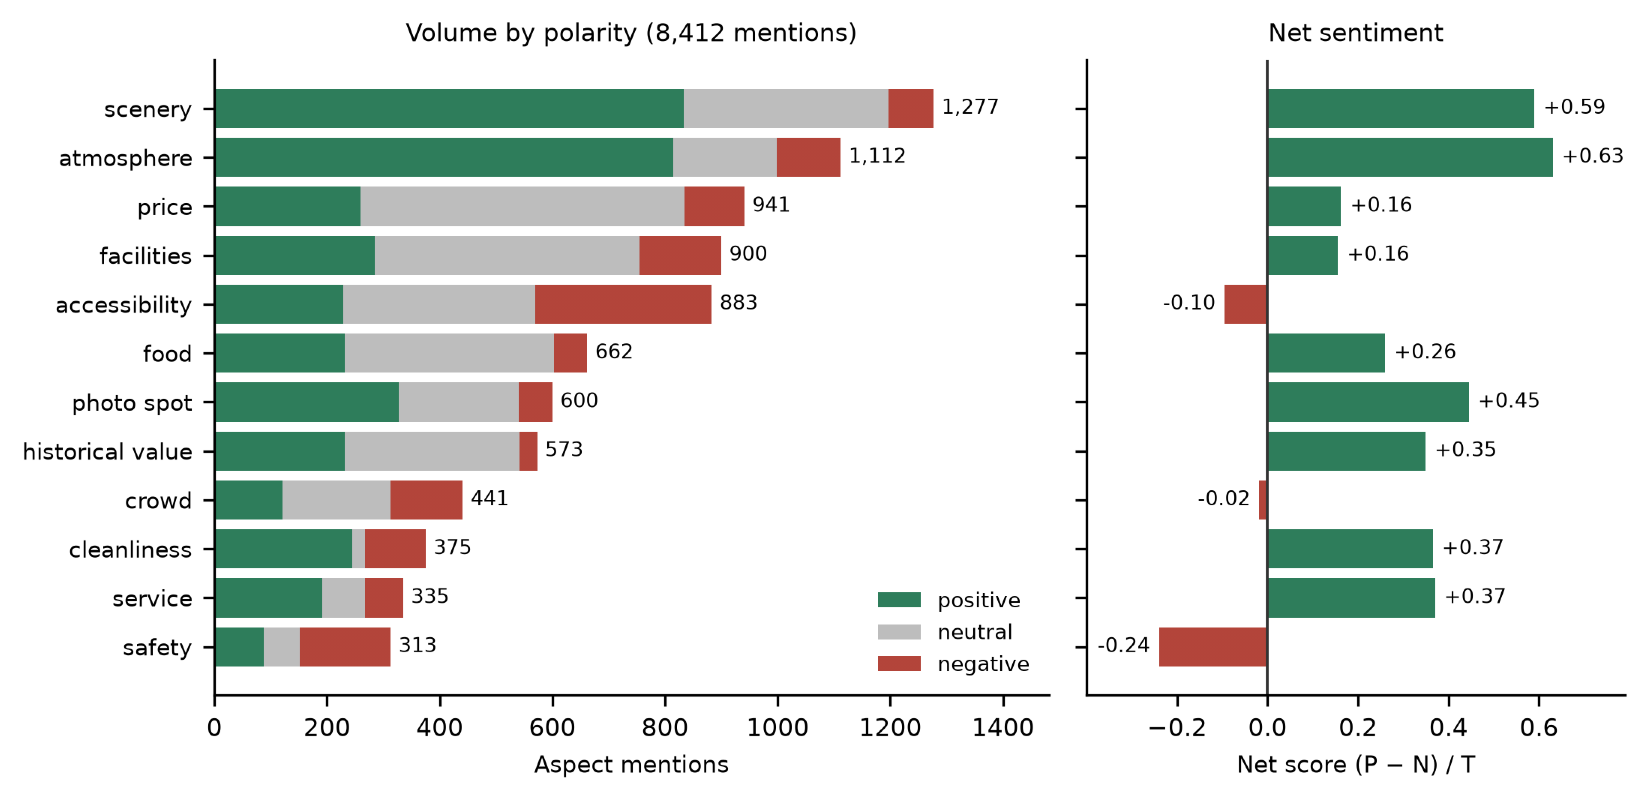
\includegraphics[width=\textwidth]{figures/fig7_aspects.pdf}
\caption{Aspect mentions by polarity (left) and net sentiment score per aspect (right).}\label{fig7}
\end{figure}

\begin{figure}[htbp]
\centering
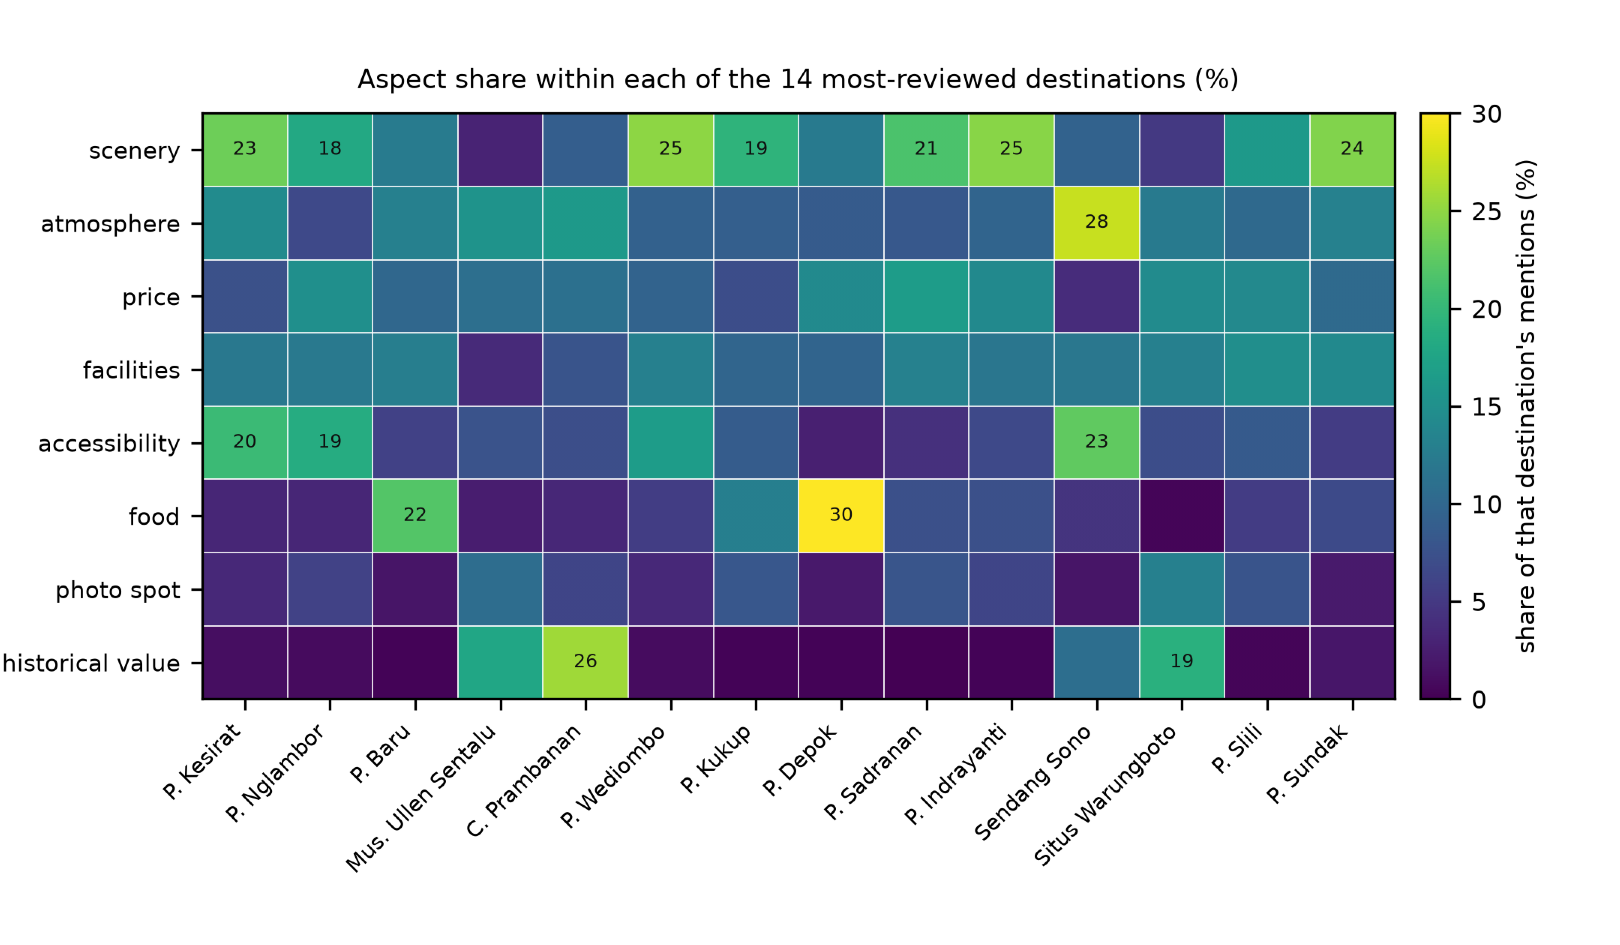
\includegraphics[width=\textwidth]{figures/fig8_aspect_destination.pdf}
\caption{Share of each destination's aspect mentions taken by the eight most frequent aspects, for the 14 most-reviewed destinations. Cells are labelled where the share reaches 18\%; each column sums to 100\%.}\label{fig8}
\end{figure}

\subsubsection{Sentences without an aspect label}\label{subsec7}

Of the 1,309 sentences without an aspect, 1,205 received an empty aspect list from the model and 104 named an aspect outside the closed taxonomy. The 1,205 are not a residual to be filled: 841 (64.2\%) are descriptive statements with no evaluative marker, 184 (14.1\%) mention aspect vocabulary without evaluating it, 159 (12.1\%) are shorter than three words, 109 (8.3\%) contain an evaluative cue whose target is the visit as a whole rather than any of the twelve aspects, and 16 (1.2\%) are questions. Labelling these as neutral would conflate ``no aspect to evaluate'' with ``evaluated as neutral'', two states the dataset must keep apart.

For the 104 sentences whose aspect fell outside the taxonomy, the model had already returned a polarity alongside the rejected aspect; that polarity is retained in a separate table without an aspect: 60 positive, 27 neutral, 14 negative and 3 mixed. These mentions are excluded from all aspect statistics reported here. The negative subset is small but substantive, containing statements such as ``Parah bgt sih.'' and a reviewer who would not recommend a beach for swimming at all. They are reported because discarding them would understate dissatisfaction that the aspect taxonomy cannot index.

\section{Discussion}\label{sec5}

\subsection{Interpretation of Topic Modelling Results}\label{subsec8}

The four thematic groupings identified by BERTopic---coastal and marine experiences, urban and photography-oriented activities, cultural heritage, and pilgrimage---reflect Yogyakarta's established identity as a multidimensional tourism destination. The thematic coherence of the discovered clusters, evidenced by a $c_v$ of 0.5912, demonstrates that BERTopic with multilingual Sentence-BERT embeddings can meaningfully segment Indonesian-language tourism discourse without the need for manually labelled topic categories. This represents a notable advancement over traditional LDA-based approaches, which rely on bag-of-words representations and are known to struggle with semantic coherence in short, noisy texts.

The outlier rate of 5.5\% is low for BERTopic on user-generated content, where review brevity and mixed-topic expression frequently prevent clean cluster assignment and outliers routinely exceed a quarter of the corpus. The improvement here is attributable to the reduced corpus size after destination filtering and to tuning \texttt{min\_cluster\_size}, which was tuned over ten candidate configurations and set to the coverage-oriented configuration reported here rather than to the coherence maximum, which left 57.2\% of reviews unassigned. Of the 84 outliers, most are very short reviews that name a single attraction without describing it, and they were retained rather than forcibly assigned. Topic coverage of 94.5\% means the topic and aspect views described in Sections~\ref{subsec5} and~\ref{subsec6} rest on almost the whole corpus.

\subsection{Interpretation of Aspect Sentiment Results}\label{subsec9}

The central finding is not that the LLM detects sentiment more accurately than earlier methods; no human-annotated gold standard was constructed, so no accuracy claim is made. The finding is structural. At review level the corpus looks overwhelmingly positive: 70.3\% of the 5,691 review-level mentions are positive against 13.4\% negative. At sentence level the same corpus yields 45.8\% positive, 16.4\% negative and 37.8\% neutral over 8,412 mentions. The negativity was present in the reviews all along; a single label per review distributed it across whatever the model happened to select. Nothing about the data changed between the two rows of Table~\ref{tab5}. Only the unit of analysis did, and that is the contribution this paper claims.

The dominant positive sentiment toward scenery/view and atmosphere, both rated ``Excellent'' per the scoring framework in Table~\ref{tab4}, corroborates prior ABSA research on tourism reviews, which consistently identifies aesthetic and environmental quality as the primary drivers of visitor satisfaction. Mehraliyev et al.\ \cite{bib24} noted in their thematic review that sensory and atmospheric aspects routinely attract the highest positive sentiment volumes across hospitality and tourism review datasets, a pattern that holds strongly in this Yogyakarta corpus. The similarly high scores for photo spots and historical/cultural value further reflect Yogyakarta's competitive advantage as a destination combining natural beauty, Instagrammable locations, and well-preserved cultural heritage, an asset combination that Li et al.\ \cite{bib14} identify as a key predictor of sustained destination popularity in the review era.

This has a practical consequence for destination managers. A dashboard built on review-level scores would report safety as adequate ($+0.088$ at review level) while 51.8\% of safety mentions are negative and concentrated at beach sites. The sentence-level figure identifies where the problem is, not merely that the destination is liked overall. The same applies to accessibility, where 313 of 883 mentions are negative but the review-level aggregate is positive ($+0.204$), and to crowd level, whose near-zero net score conceals opposed experiences rather than indifference ($+0.141$ at review level).

The magnitude of the shift varies by aspect and is largest where the review carries genuinely mixed content. Facilities moves from $+0.613$ at review level to $+0.156$ at sentence level, food and beverage from $+0.652$ to $+0.260$, and historical value from $+0.721$ to $+0.349$. These aspects are frequently mentioned in passing inside reviews whose overall tone was set by something else, so the review-level score reports the surrounding sentence rather than the aspect itself. Only cleanliness is stable ($+0.322$ to $+0.365$), which is consistent with it being mentioned mostly in sentences of its own.

Compared to Nawawi et al.\ \cite{bib5}, whose zero-shot RoBERTa-based ABSA on Indonesian tourism reviews identified analogous aspect categories, the present study's Qwen2.5-7B-Instruct approach produces a verbatim keyword-level evidence trail per aspect, enabling a more targeted diagnostic interpretation. This is consistent with the finding of Zhang et al.\ \cite{bib19} that structured aspect extraction remains more demanding for LLMs than coarse polarity, and with Krugmann and Hartmann \cite{bib18}, who showed that instruction-tuned LLMs can approach fine-tuned classifiers on domain-specific sentiment tasks without requiring annotated training data.

Aspect composition also varies across destinations (Fig.~\ref{fig8}), with no regional average describing any of them: at Candi Prambanan 25.7\% of aspect mentions concern historical value, whereas pooled across the five most-reviewed beaches scenery leads at 19.7\%; the same holds for landmark destinations that fall outside that panel: in Malioboro's 142 aspect mentions atmosphere and crowd level account for 25.4\% and 19.0\%, and in Tugu Jogja's 198, atmosphere and photo spots for 24.7\% and 19.2\%. Because these are composition shares within a destination, they are descriptive and carry no inference about destination quality.

Among the aspects above the ``Good'' threshold, facilities ($+0.156$) is noteworthy for receiving the fourth-highest mention volume (900) while recording one of the lowest positive scores. This combination of high engagement and a lower score suggests that visitors are strongly interested in facilities-related content, but the experience is less consistent than for the top-rated aspects. This underscores the value of examining both the sentiment score and the raw mention count in tandem when prioritising improvement areas, rather than relying on either metric in isolation.

\subsection{Limitations}\label{subsec10}

Four limitations constrain these findings. First, the dataset is restricted to Google Maps reviews, which introduces platform sampling bias: users of this platform skew toward smartphone-literate, locally connected visitors and may underrepresent international tourists and older demographics. Second, the high five-star rate (78.6\%) and mean rating (4.68/5) indicate a positive-skew bias in the source, which inflates positive sentiment proportions and makes the negative aspects reported here conservative rather than exaggerated. Third, the closed 12-aspect taxonomy means any dimension outside it is systematically absent; 104 sentences in this corpus named such an aspect, and their polarity was retained only without an aspect. Fourth, the scope is confined to Yogyakarta, and 18 of the 34 destinations are beaches, so the coastal concentration of safety concerns reflects the sampling frame as well as the destination. No human-annotated gold standard was constructed, so the extraction is evaluated for internal consistency and evidence grounding rather than against external labels.

\subsection{Recommendations for Future Research}\label{subsec11}

Based on the findings and limitations of this study, the following methodological recommendations are offered for researchers pursuing similar analyses. First, multi-platform data integration combining Google Maps with TripAdvisor, Traveloka, and social media would substantially reduce platform sampling bias and improve demographic representativeness of the review corpus. Second, longitudinal or time-series ABSA designs are recommended to detect seasonal and event-driven sentiment fluctuations, as static cross-sectional analysis cannot capture the temporal dynamics of visitor satisfaction. Third, there is a need to systematically evaluate the performance of other multilingual LLMs in handling complex linguistic features specific to Indonesian user-generated content, including sarcasm, irony, and dense code-switching between Bahasa Indonesia and English. Fourth, future studies should explore dynamic or data-driven aspect taxonomies---for example, using BERTopic-derived clusters to inductively generate aspect categories rather than predefining them---to reduce the risk of missing emerging or destination-specific experiential dimensions. Fifth, expanding the framework to other Indonesian priority destinations and to international tourism contexts would test the generalisability of both the methodology and the specific aspect sentiment patterns identified here, enabling cross-regional comparative analyses that could inform national-level tourism strategy.

\section{Conclusions}\label{sec6}

This study examined whether the unit of analysis changes what a tourism review corpus can reveal. Splitting 1,530 Google Maps reviews from 34 Yogyakarta destinations into 6,479 labelled sentences and extracting aspects at that level produced 8,412 mentions, 1.48 times the review-level yield from the same corpus. The additional structure is not noise: 33.1\% of sentences discuss two or more aspects, 19.2\% of those are internally contradictory, and 42.3\% of reviews carry competing polarities. Re-extraction at sentence level reverses the sign of three aspects, with safety ($-0.24$), accessibility ($-0.10$) and crowd level ($-0.02$) net negative where review-level aggregation scored them positive.

The primary contribution is evidence that aggregation, not model capability, governs what is visible in review analytics. A pipeline that assigns one label per review will report destination satisfaction accurately at the aggregate level and misreport specific operational problems. Sentence-level extraction with a closed aspect taxonomy and verbatim evidence grounding resolves this without requiring annotated training data, and the approach transfers to any domain where a single text carries mixed evaluations.

Despite its contributions, this study is subject to limitations relating to single-platform data collection, positivity bias in the source reviews, the use of a closed 12-aspect taxonomy that may not capture all relevant experiential dimensions, and geographic confinement to Yogyakarta, which limits the direct generalisability of the findings to other destinations. Future work should build on this framework by broadening data collection across platforms and regions, incorporating temporal sentiment analysis, benchmarking multilingual LLMs for sarcasm and code-switching in Indonesian text, exploring dynamic aspect taxonomies, and replicating the approach across diverse tourism destinations to develop a generalisable national tourism intelligence system.

\backmatter

\bmhead{Acknowledgements}

The authors thank the Department of Informatics, Universitas Islam Indonesia, for supporting this research.

\section*{Declarations}

\begin{itemize}
\item \textbf{Funding.} This research received no specific grant from any funding agency in the public, commercial, or not-for-profit sectors.
\item \textbf{Competing interests.} The authors declare no competing interests. No funding body had any role in the design of the study, the collection, analysis, or interpretation of data, or in the writing of the manuscript.
\item \textbf{Ethics approval and consent to participate.} Not applicable. This study analysed publicly available online reviews; no human subjects were involved and no personal data were collected beyond what reviewers published publicly.
\item \textbf{Consent for publication.} Not applicable.
\item \textbf{Data availability.} The review dataset and the extraction outputs that support the findings of this study are available from the corresponding author upon reasonable request. The corpus contains user-generated content published on Google Maps; to respect reviewer privacy, usernames are not redistributed.
\item \textbf{Materials availability.} Not applicable.
\item \textbf{Code availability.} The pipeline code (sentence splitter, aspect extraction, aggregation and analysis scripts) is available from the corresponding author upon reasonable request.
\item \textbf{Author contribution.} A.F.H.: Conceptualisation, Data curation, Investigation, Methodology, Supervision, Writing -- original draft, Writing -- review and editing. A.A.A.: Data curation, Writing -- original draft. A.A.: Data curation, Writing -- original draft. Ardiansyah: Methodology, Writing -- review and editing. All authors have read and agreed to the published version of the manuscript.
\end{itemize}

\bibliography{sn-bibliography}

\end{document}
